\section{Durchführung}
\label{sec:Durchführung}
In der Durchführung des Versuchs wird zuerst eine Schaltung aufgebaut mit deren Hilfe die generelle Funktionsweise eines Lock-In-Verstärkers untersucht wird. Im zweiten Versuchsteil wird eine Photodetektorschaltung aufgebaut, mit der die Rauschunterdrückung des Lock-In-Verstärkers untersucht wird.
\subsection{Untersuchung der Funktionsweise eines Lock-In-Verstärkers}
Der schmatische Aufbau der genutzten Schaltung für die Untersuchung der Funktionsweise eines Lock-In-Verstärkers ist in \autoref{fig:schema2} dargestellt.
\begin{figure}[H]
    \centering
    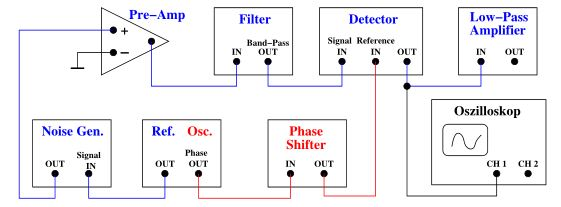
\includegraphics{images/schema2.JPG}
    \caption{Schematischer Aufbau der Messschaltung zur Untersuchung der Funktionsweise eines Lock-In-Verstärkers. \cite{sample}}
    \label{fig:schema2}
\end{figure}
\noindent
Zur praktischen Realisierung der Schaltung aus \autoref{fig:schema2} wird die Apparatur aus \autoref{fig:app} genutzt.
\begin{figure}[H]
    \centering
    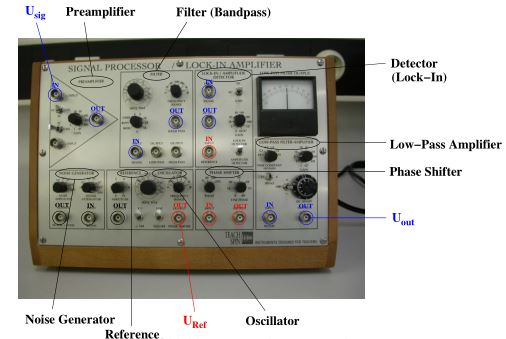
\includegraphics{images/schaltung.JPG}
    \caption{Schaltapparatur für die Realisierung eines Lock-In-Verstärkers. \cite{sample}}
    \label{fig:app}
\end{figure}
\noindent
\subsection{Überprüfen der Rauschunterdrückung}
\begin{figure}[H]
    \centering
    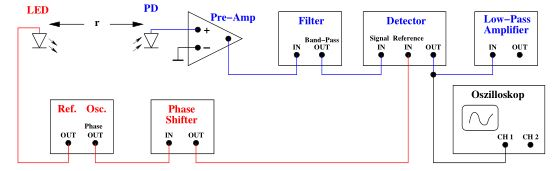
\includegraphics{images/photo.JPG}
    \caption{Schematischer Aufbau der Photodetektorschaltung zur Untersuchung der Rauschunterdrückung. \cite{sample}}
    \label{fig:photo}
\end{figure}
\noindent